\begin{frame}{Cette semaine}
  Avec un.e partenaire, discutez de ce que vous avez fait cette semaine.
  Utilisez le \emph{passé composé} puisque ces acitivtés ont eu lieu dans le passé.
  \begin{columns}
    \column{0.5\textwidth}
      \begin{center}
        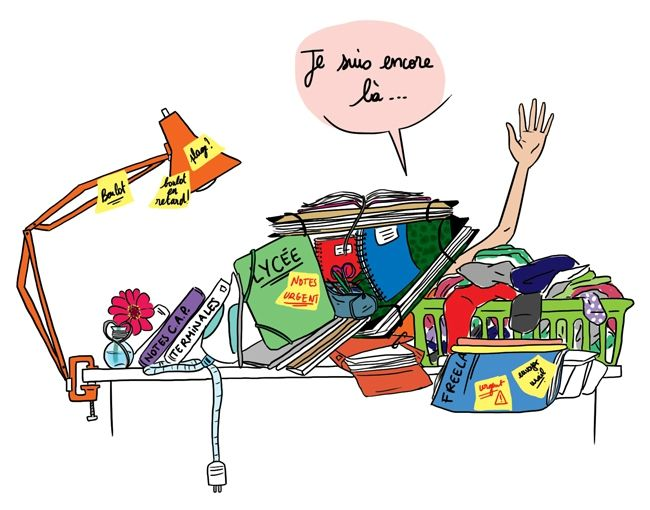
\includegraphics[scale=0.25]{débordé.jpg}
      \end{center}
    \column{0.5\textwidth}
      \only<1>{
        \begin{itemize}
          \item[] \textbf{Modèle:}
          \item[E1:] Lundi, je suis allé à l'épicerie. J'ai acheté de la viande, parce que j'ai cuisiné un repas plus tard.
          \item[E2:] Moi, je ne cuisine jamais. Alors, mardi j'ai déjeuné à Clocked, et ensuite j'ai voté à l'hôtel de ville.
        \end{itemize}
      }
      \only<2->{
        Maintenant, écrivez un paragraphe avec les détails de votre semaine que vous venez de donner à votre partenaire.
      }
  \end{columns}
\end{frame}